\newpage
\section{Use Case Diagrams}
\label{sec:UseCaseDiagrams}

This diagram shows the general functionality of our system where the primary actor is the Archiver. 

\begin{figure}[ht]
\begin{center}
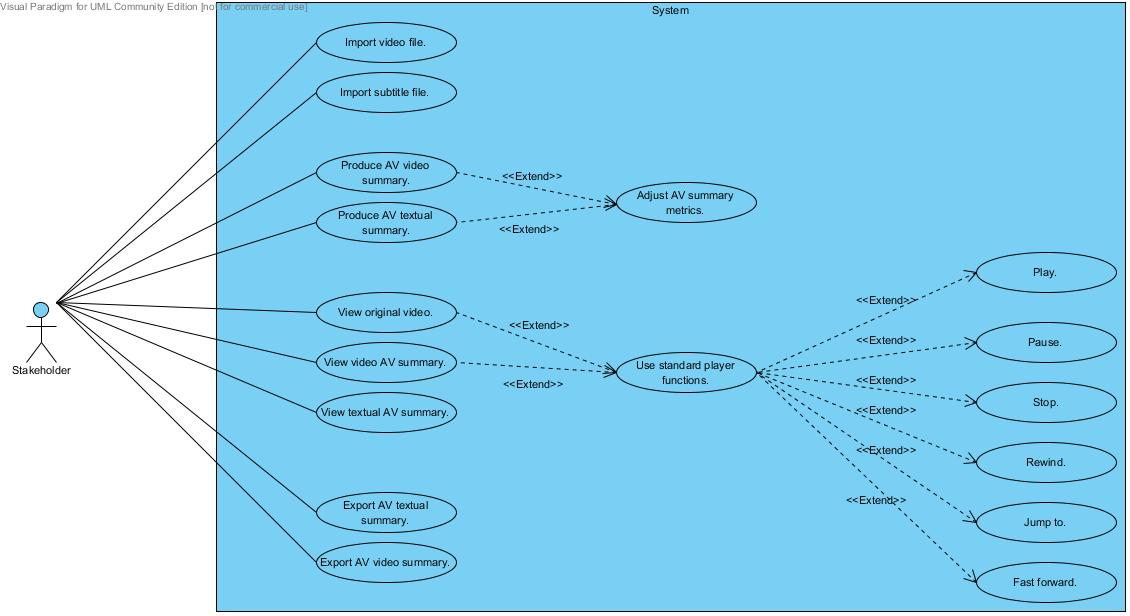
\includegraphics[trim = 0mm 0mm 0mm 0mm, clip, scale=0.38]{Images/general_use_case_diagram.jpg}
\end{center}
\caption{General Use Case Diagram}
\end{figure}

This diagram depicts the senarios of the Archive Monetisation, Rights Assessment and Archive Content Selection problems described in section \ref{sec:ProjectProblem}:

\begin{figure}[ht]
\begin{center}
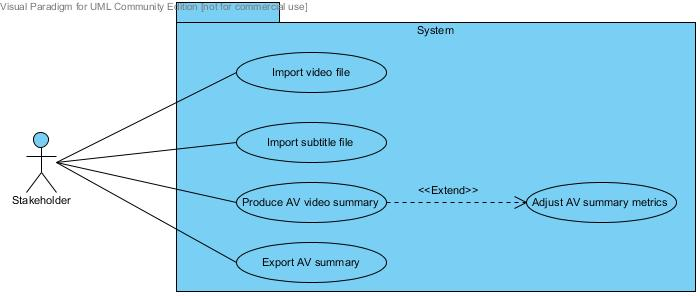
\includegraphics[trim = 0mm 0mm 0mm 0mm, clip, scale=0.61]{Images/archive_monetisation_use_case_diagram.jpg}
\end{center}
\caption{Archive Monetisation Diagram}
\end{figure}

\newpage
\begin{figure}[ht]
\begin{center}
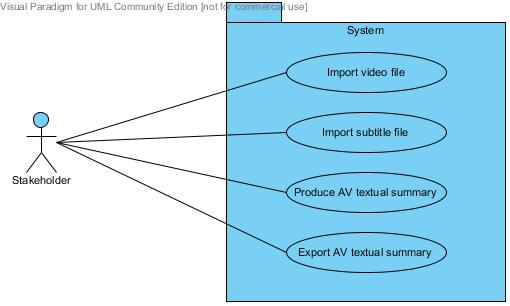
\includegraphics[trim = 0mm 0mm 0mm 0mm, clip, scale=0.75]{Images/rights_assessment_use_case_diagram.jpg}
\end{center}
\caption{Rights Assessment Diagram}
\end{figure}

\begin{figure}[ht]
\begin{center}
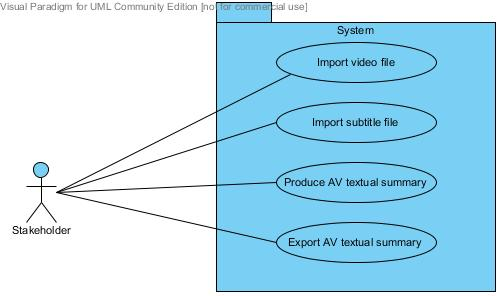
\includegraphics[trim = 0mm 0mm 0mm 0mm, clip, scale=0.75]{Images/archive_content_selection_use_case_diagram.jpg}
\end{center}
\caption{Archive Content Selection Diagram}
\end{figure}
